\chapter{Installazione e accesso}


\section{Requisiti di sistema}
\label{Requisiti sistema}
Di seguito sono riportati i requisiti minimi per utilizzare il software MegAlexa:

\begin{itemize}
	\item \textbf{Sistema Operativo}:\glossario{Android}4.4 KitKat API 19;
	\item \textbf{Memoria richiesta}: 50MB;
	\item \textbf{Connessione internet}: Richiesta;
	\item \textbf{Dispositivo}: Amazon \textit{Echo$_{G}$};
	\item \textbf{Applicazione Amazon Alexa installata};
	\item \textbf{Applicazione MegAlexa installata}.
\end{itemize}

\textbf{NOTA BENE:} si consiglia fortemente l'utilizzo di un dispositivo Amazon Echo per un'esperienza migliore. Se non si è in possesso di tale dispositivo c'è la possibilità di acquistarlo sul sito di \href{https://www.amazon.it}{Amazon}.

\section{Installazione applicazione}
Scaricare e installare le \glossario{applicazioni} Amazon Alexa e MegAlexa dal Google \href{https://play.google.com/store/apps?hl=it}{Play Store} sul proprio dispositivo mobile.
\newpage
\section{Avvio applicazione MegAlexa}
\label{Installazione MegAlexa}
Avviare l'applicazione ed effettuare il login con il proprio\glossario{account}Amazon cliccando sul tasto "Login with Amazon".

\begin{figure}[!ht]
	\centering
	\fbox{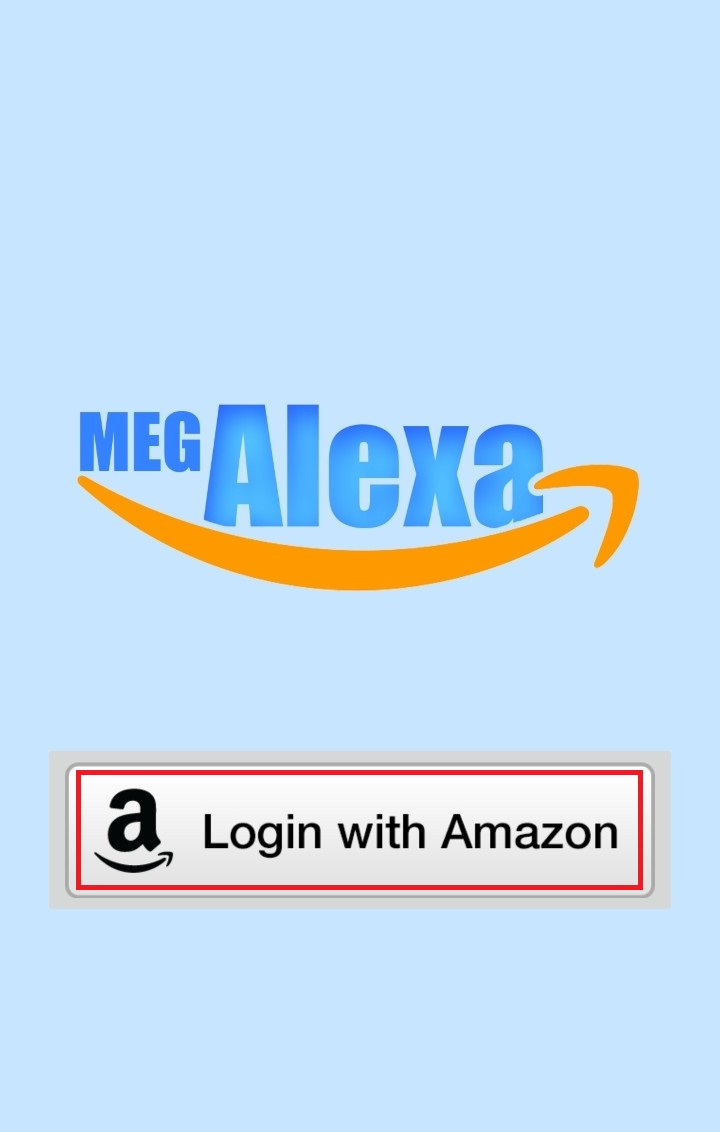
\includegraphics[scale=0.2]{images/Login.jpg}}
	\caption{Schermata principale app}
\end{figure}

\subsection{Login con account Amazon}

\begin{enumerate}
\item Se non si possiede un account Amazon cliccare sul tasto "Crea un nuovo account Amazon" e seguire la procedura guidata per creare un nuovo account.
\item Se si possiede un account Amazon:
\begin{enumerate}
	\item Inserire le credenziali del proprio account Amazon;
	\item Cliccare su "Accedi" per effettuare il login.
\end{enumerate}
\begin{figure}[!ht]
	\centering
	\fbox{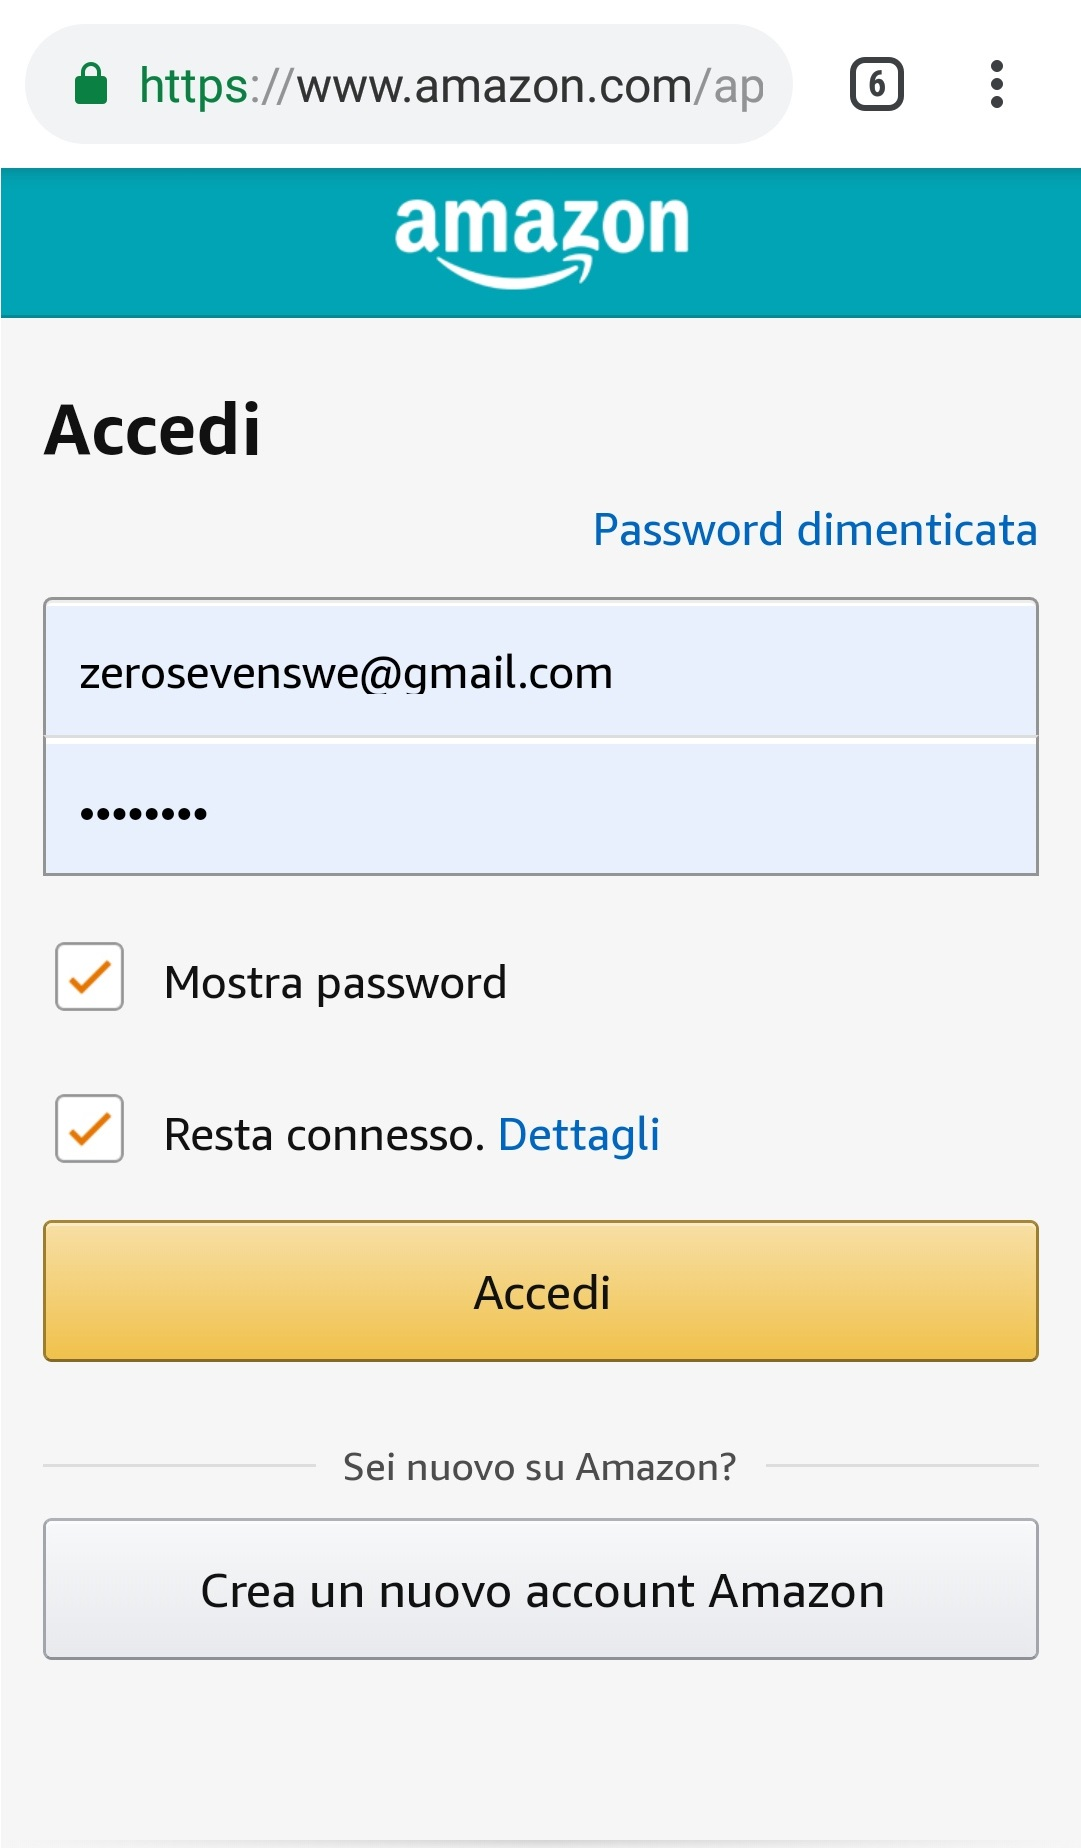
\includegraphics[scale=0.2]{images/Autentication.jpg}}
	\caption{Login ad Amazon}
\end{figure}
\end{enumerate}
\newpage
\subsection{Logout}
\begin{enumerate}
	\item Dalla schermata di elenco dei workflow, scorrere il dito dall'estrema sinistra della schermo a destra per far comparire il menù laterale;
	\begin{figure}[!ht]
		\centering
		\fbox{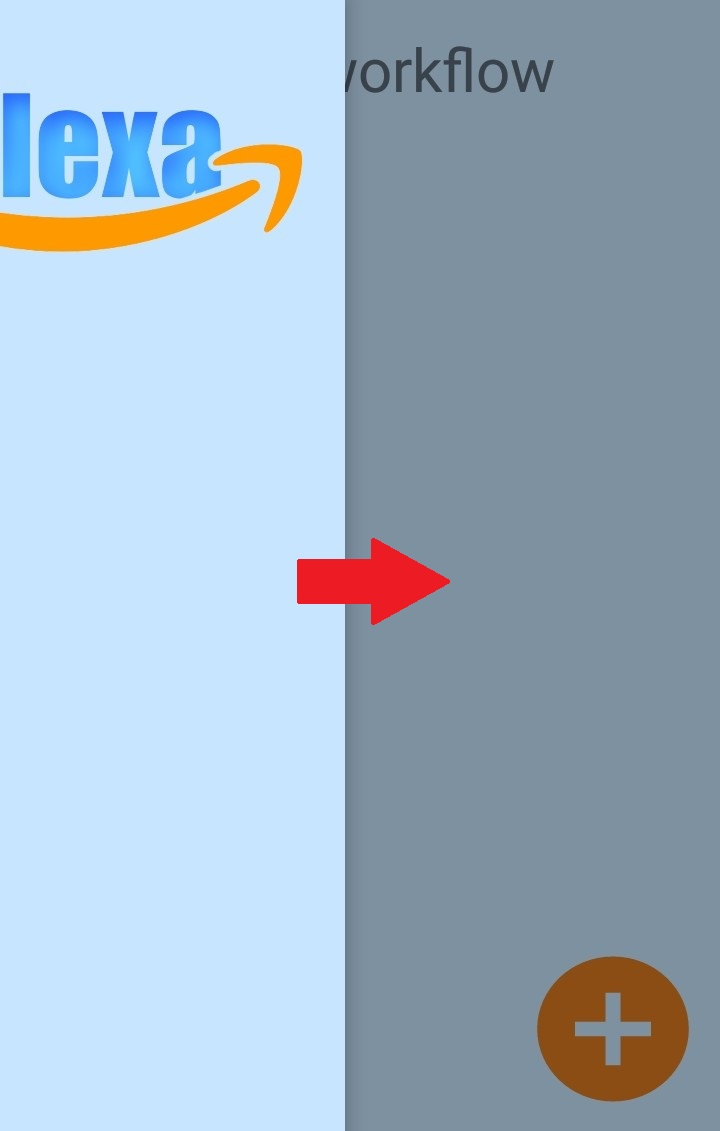
\includegraphics[scale=0.2]{images/SwipeLeftToRight.jpg}}
		\caption{Apparizione menù laterale}
	\end{figure}
\newpage
	\item Cliccare sul tasto "Exit" per effettuare il logout dall'applicazione.
	\begin{figure}[!ht]
		\centering
		\fbox{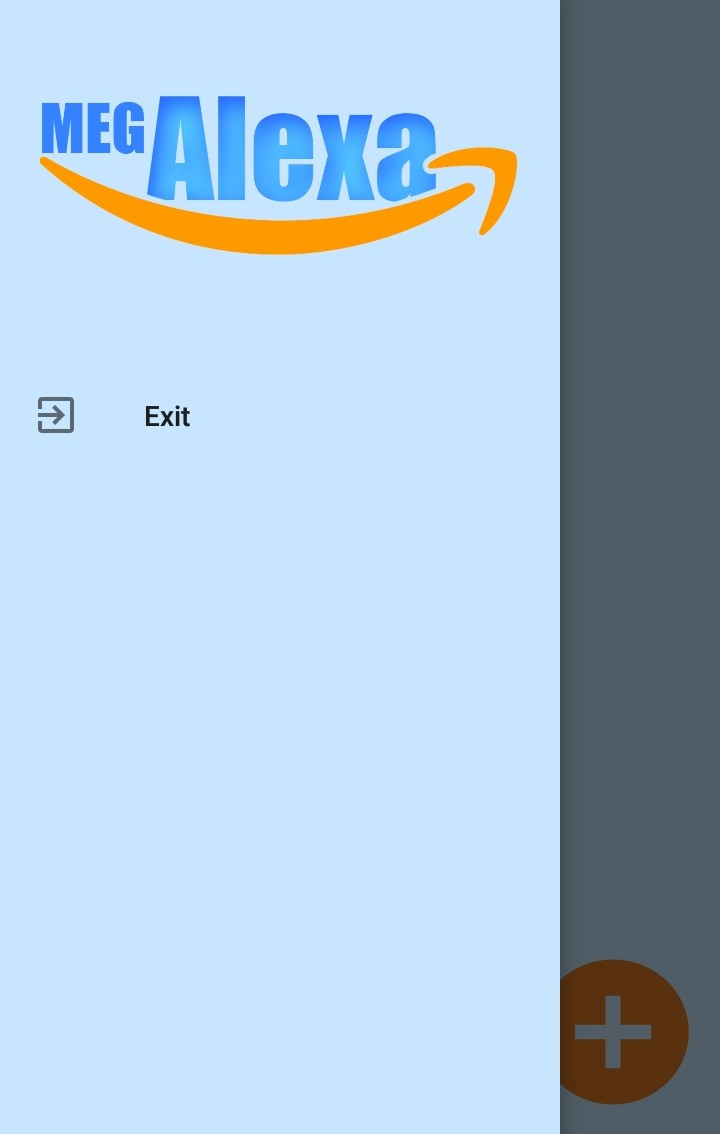
\includegraphics[scale=0.2]{images/Logout.jpg}}
		\caption{Logout}
	\end{figure}
\end{enumerate}

\newpage
\section{Avvio applicazione Amazon Alexa}
\label{Avviso Amazon Alexa}
\subsection{Login Amazon Alexa}
\begin{enumerate}
\item Avviare l'\glossario{applicazione} Amazon Alexa sul dispositivo mobile;
\item Inserire le credenziali dell'account Amazon; 
\item Cliccando sul tasto "Accedi".
\end{enumerate}
\begin{figure}[H]
	\centering
	\includegraphics[width=0.5\textwidth]{images/accessoAlexa.png}
	\caption{Login applicazione Amazon Alexa}
\end{figure}

\begin{itemize}
 \item  Se non si possiede un \glossario{account} Amazon cliccare sul tasto "Crea un nuovo account Amazon" e seguire le successive istruzioni per creare un nuovo account.
 \end{itemize}
 

\subsection{Logout Amazon Alexa}
\begin{enumerate}
\item Dalla schermata "Home" schiacciare sul pulsante menù in alto a sinistra contrassegnato da tre linee orizzontali;

\begin{figure}[H]
	\centering
	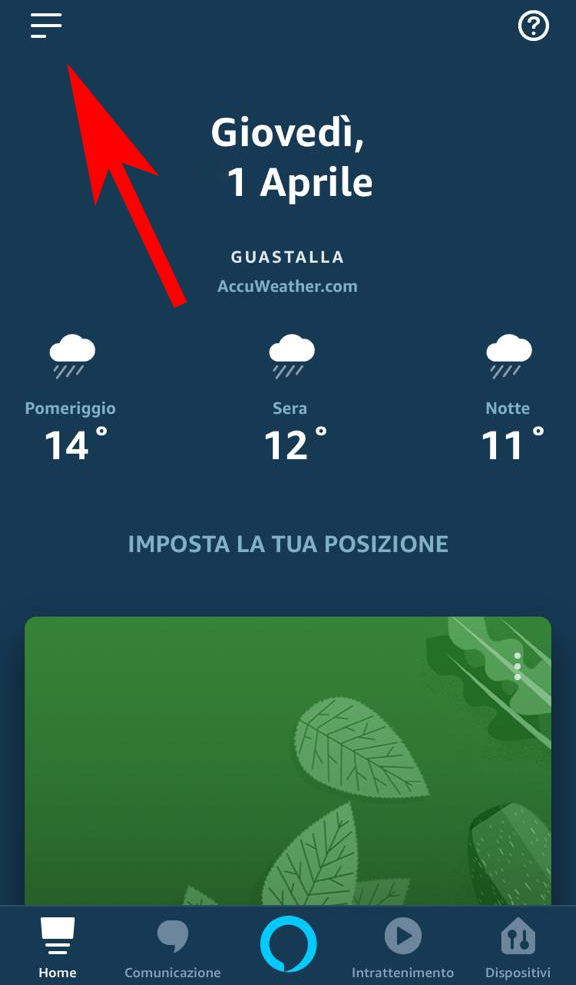
\includegraphics[width=0.5\textwidth]{images/MenuAlexa.png}
	\caption{Menu nell'applicazione Amazon Alexa}
\end{figure}

\newpage
\item Si aprirà una barra laterale sulla sinistra. In fondo a questa barra laterale schiacciare sulla voce "Impostazioni";

\begin{figure}[H]
	\centering
	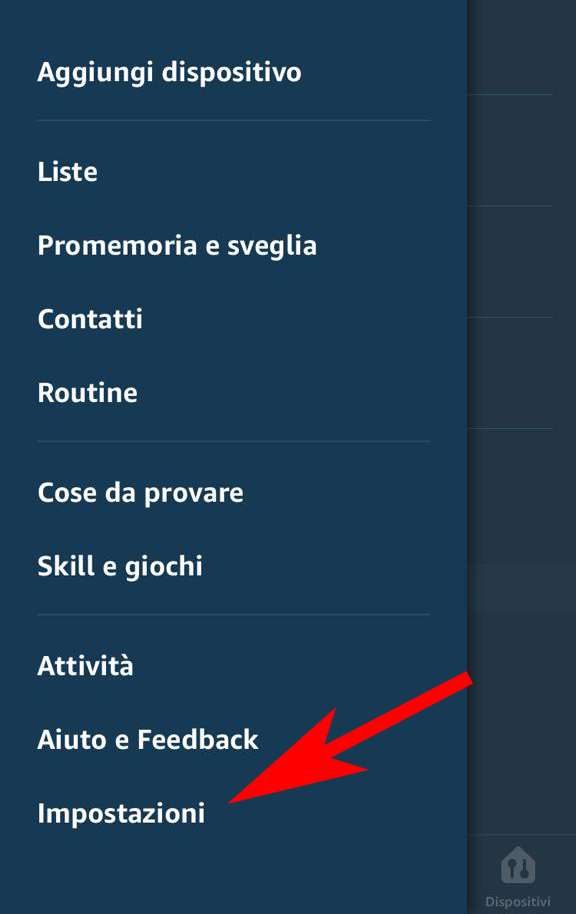
\includegraphics[width=0.5\textwidth]{images/ImpostazioniAlexa.png}
	\caption{Barra laterale Amazon Alexa}
\end{figure}

\newpage
\item Sulla  nuova schermata in basso si trova la voce "Esci", schiacciare se si vuole eseguire il logout;

\begin{figure}[H]
	\centering
	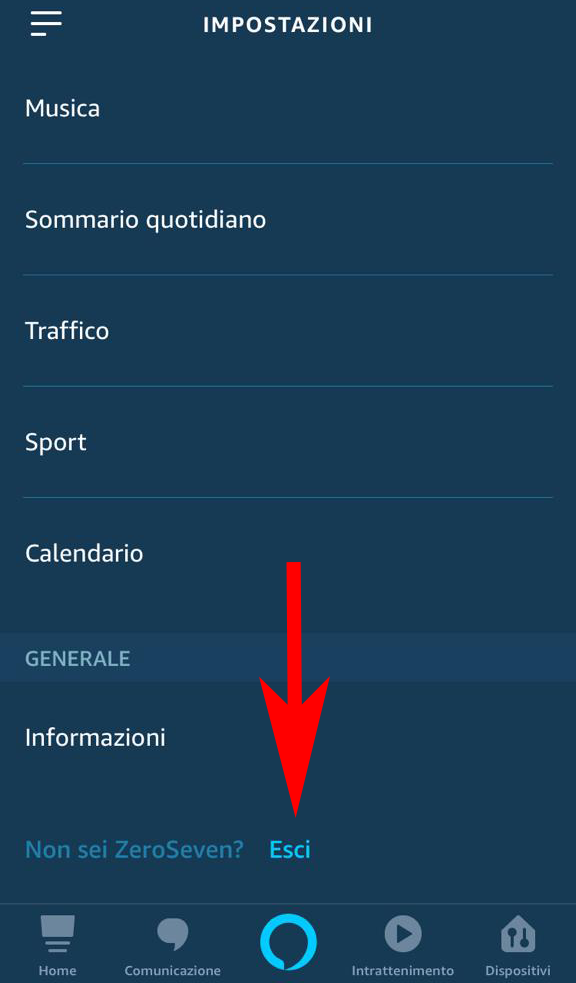
\includegraphics[width=0.5\textwidth]{images/LogoutAlexa.png}
	\caption{Esci nell'applicazione Amazon Alexa}
\end{figure}

\item Logout completato.
\end{enumerate}

 
 








